\documentclass[12pt,a4paper]{article}
\usepackage{bold-extra}
\usepackage{appendix}
\usepackage{amsfonts,amsmath,amssymb}
\usepackage{enumerate}
\usepackage{float}
\usepackage{geometry}
\usepackage{graphicx}
\usepackage{latexsym}
\usepackage{listings}
\usepackage{multicol,multirow}
\usepackage{subfigure}
\usepackage{tabularx}
\usepackage{ulem}
\usepackage{tikz}
\usetikzlibrary{angles,quotes}
\usepackage{verbatim}
\usepackage{xcolor}
\geometry{a4paper,left=1in,right=1in,top=1in,bottom=1in}
\begin{document}
\centerline{\Huge{{\textbf{PHYSICS II\ \ Problem Set 2}}}}
\vspace{0.5cm}
\leftline{\large{Name: Haotian Fu}}
\rightline{\large{Student ID: 520021910012}}
\section*{\large \textbf{Problem 1}}~{\textbf{Solution}}

\begin{enumerate}[(a)]
    \item According to
    \begin{align}
        \oint_{\Sigma} \mathbf{E}_{G} \hat{n} d A=-4 \pi G M_{\Sigma}
        \label{Gravitation}
    \end{align}
    we may express the information we have already known as 
    \begin{align}
        \mathbf{E}_{G} \cdot 4\pi r^2 = -4\pi GM
    \end{align}
    Hence
    \begin{align}
        \mathbf{E}_{G} = -\frac{GM}{r^2}
    \end{align}
    
    \item 
    \begin{enumerate}[i)]
        \item $r > R$ \\
        Every part of the uniform solid ball is within the radius $r$, thus $M_{\Sigma} = M$. \\
        According to Eq.(\ref{Gravitation}), we know
        \begin{align}
            &\mathbf{E}_{G} \cdot 4\pi r^2 = -4\pi GM \\
            \Rightarrow\quad &\mathbf{E}_{G} = -\frac{GM}{r^2}
        \end{align}
        
        \item $r < R$ \\
        Only parts with radius $r < R$ has the \textbf{effective mass} $\frac{r^3}{R^3} M$. \\
        Hence we get the following equation according to Eq.(\ref{Gravitation})
        \begin{align}
            &\mathbf{E}_{G} \cdot 4\pi r^2 = -4\pi G \cdot \frac{r^3}{R^3}M \\
            \Rightarrow\quad &\mathbf{E}_{G} = -\frac{GMr}{R^3}
        \end{align}
    \end{enumerate}
    
    \item we will still discuss this problem by two parts correspondingly.
\begin{enumerate}[i)]
    \item $r > R$ \\
    Every part of the uniform solid ball is within the radius $r$, thus $M_{\Sigma} = M$. \\
    According to Eq.(\ref{Gravitation}), we know
    \begin{align}
        &\mathbf{E}_{G} \cdot 4\pi r^2 = -4\pi GM \\
        \Rightarrow\quad &\mathbf{E}_{G} = -\frac{GM}{r^2}
    \end{align}
    
    \item $r < R$ \\
    Since there is no mass within the ball, $M_{\Sigma} = 0$. \\
    Hence
    \begin{align}
        \mathbf{E}_{G} = 0
    \end{align}
\end{enumerate}
\end{enumerate}

\section*{\large \textbf{Problem 2}}~{\textbf{Solution}}

\begin{enumerate}[(a)]
    \item Suppose the Gaussian surface is the surface of this region. We may first calculate the electric flux of this region.
    \begin{align}
        \Phi_E = \oint\limits_{\Sigma} \overline{E} \circ d\overline{A} = \oint\limits_{\Sigma} E_{\perp} dA
    \end{align}
    Since Gaussian surface is a certain region in one space, the total electric field has both inward and outward, cancelling each other out.
    
    Hence
    \begin{align}
        \Phi_E = 0
    \end{align}
    
    Besides, according to \textbf{Gauss's Law}
    \begin{align}
        \Phi_E = \frac{q_{encl}}{\varepsilon_0}
    \end{align}
    
    Therefore
    \begin{align}
        q_{encl} = 0
    \end{align}
    Namely, this region of space must be electrically neutral.
    
    \item The converse is \textbf{TRUE} since if there is no charge inside Gaussian surface, there will not be any electric flux passing through it.
\end{enumerate}

\section*{\large \textbf{Problem 3}}~{\textbf{Solution}}

Suppose the cube given in this problem has the side length $a$. Imagine the point charge is in the center of a cube whose side length is $2a$. Then according to \textbf{Gauss's Law}, the electric flux of this $2a$-cube is
$$
    \frac{Q}{\varepsilon_0}
$$
since the point charge is completely within this cube.

According to the symmetry, each surface of the cube has the electric flux
$$
    \frac{Q}{\varepsilon_0} \div 6 = \frac{Q}{6\varepsilon_0}
$$

Notice that one surface of the $2a$-cube is as four times big as the surface $ABCD$ given in this problem. Hence, the electric flux through the surface $ABCD$ can be denoted as
\begin{align}
    \Phi_E(ABCD) = \frac{1}{4} \times \frac{Q}{6\varepsilon_0} = \frac{Q}{24\varepsilon_0}
\end{align}

\section*{\large \textbf{Problem 4}}~{\textbf{Solution}}

\begin{enumerate}[(a)]
    \item
    \begin{align}
        Q = \int\limits_{ball} \rho dV = \int_a^b \rho \cdot (4\pi r^2) dr
    \end{align}
    Hence we get
    \begin{align}
        Q = 2k\pi(b^2 - a^2)
    \end{align}
    
    \item
        \begin{enumerate}[(i)]
            \item Trivially, there is no electric charge within the region where $r < a$. \\
            Thus the electric field \textbf{E} is equal to \textbf{0}.
            \item Set the spherical shell with radius $r$ as the \textbf{Gaussian surface}. Then we will calculate the quantities of charges within Gaussian surface.\\
            Based on previous problems(\textbf{Problem 3(a)}), we have
            \begin{align}
                Q^{\prime} = \int_a^r \rho \cdot (4\pi r^2) dr = \int_a^r \frac{k}{r} \cdot (4\pi r^2) dr = 2k\pi (r^2-a^2)
            \end{align}
            Hence according to \textbf{Gauss's Law}, the electric flux is
            \begin{align}
                \Phi_E(r) = \frac{Q^{\prime}}{\varepsilon_0} = \frac{2k\pi (r^2-a^2)}{\varepsilon_0}
                \label{3-Gauss's Law}
            \end{align}
            
            Meanwhile, according to the definition of \textbf{electric flux}
            \begin{align}
                \Phi_E(r) = \oint\limits_{\Sigma} \textbf{E} \circ d\textbf{A} = E(r) \cdot (4\pi r^2)
                \label{3-definition}
            \end{align}
            since the electric field is perpendicular to the spherical shell everywhere.\\
            Thus compare Eq.(\ref{3-Gauss's Law}) and Eq.(\ref{3-definition}), we get
            \begin{align}
                \frac{2k\pi (r^2-a^2)}{\varepsilon_0} = E(r) \cdot (4\pi r^2)
            \end{align}
            Hence
            \begin{align}
                E(r) = \frac{k(r^2 - a^2)}{2\varepsilon_0r^2}
            \end{align}
            pointing perpendicularly from the inner sphere to the outer sphere.
            \item According to \textbf{Gauss's Law}, the total electric flux is
            \begin{align}
                \Phi_E = \frac{Q}{\varepsilon_0} = \frac{2k\pi (b^2 - a^2)}{\varepsilon_0}
                \label{3-flux1}
            \end{align}
            According to the definition of \textbf{electric flux}
            \begin{align}
                \Phi_E = \oint\limits_{\Sigma} \textbf{E} \circ d\textbf{A} = E(r) \cdot (4\pi r^2)
                \label{3-flux2}
            \end{align}
            since the electric field is perpendicular to the spherical shell\\
            Thus compare Eq.(\ref{3-flux1}) and Eq.(\ref{3-flux2}), we get
            \begin{align}
                \frac{2k\pi (b^2 - a^2)}{\varepsilon_0} = E(r) \cdot (4\pi r^2)
            \end{align}
            Hence
            \begin{align}
                E(r) = \frac{k(b^2 - a^2)}{2\varepsilon_0 r^2}
            \end{align}
        \end{enumerate}
        Therefore, we conclude that
        \begin{align*}
            E = 
            \left\{
                \begin{array}{lcl}
                     0 & & (r < a) \\
                       \\
                     \frac{k(r^2 - a^2)}{2\varepsilon_0r^2} & & (a < r < b) \\
                       \\
                     \frac{k(b^2 - a^2)}{2\varepsilon_0 r^2} & & (r > b)
                \end{array}
            \right.
        \end{align*}
        
        \item The required plot is shown as follows.
        \begin{figure}[!htpb]
            \centering
            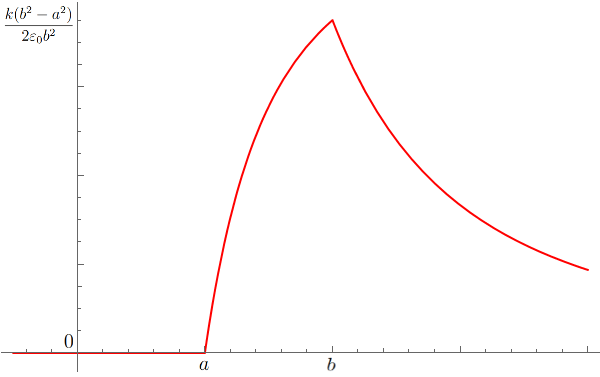
\includegraphics[width=0.5\textwidth]{hw2-p3-plot.png}
            \caption{\textbf{E} vs. $r$}
            \label{fig:3-plot}
        \end{figure}
\end{enumerate}

\section*{\large \textbf{Problem 5}}~{\textbf{Solution}}

In this problem, we may as well use \textbf{cylindrical coordinate system}$(r,\varphi,z)$ to address it. Suppose the plane composed by point P and the symmetric axis perpendicular to the base surface (denoted as \textbf{middle axis}) as $\Pi_1$ and the plane perpendicular to $\Pi_1$ through point P as $\Pi_2$(As shown in Fig. \ref{fig:4-sketch}a). Three components of \textbf{electric field} are also shown in Fig. \ref{fig:4-sketch}a.
\begin{figure}[!htpb]
    \centering
    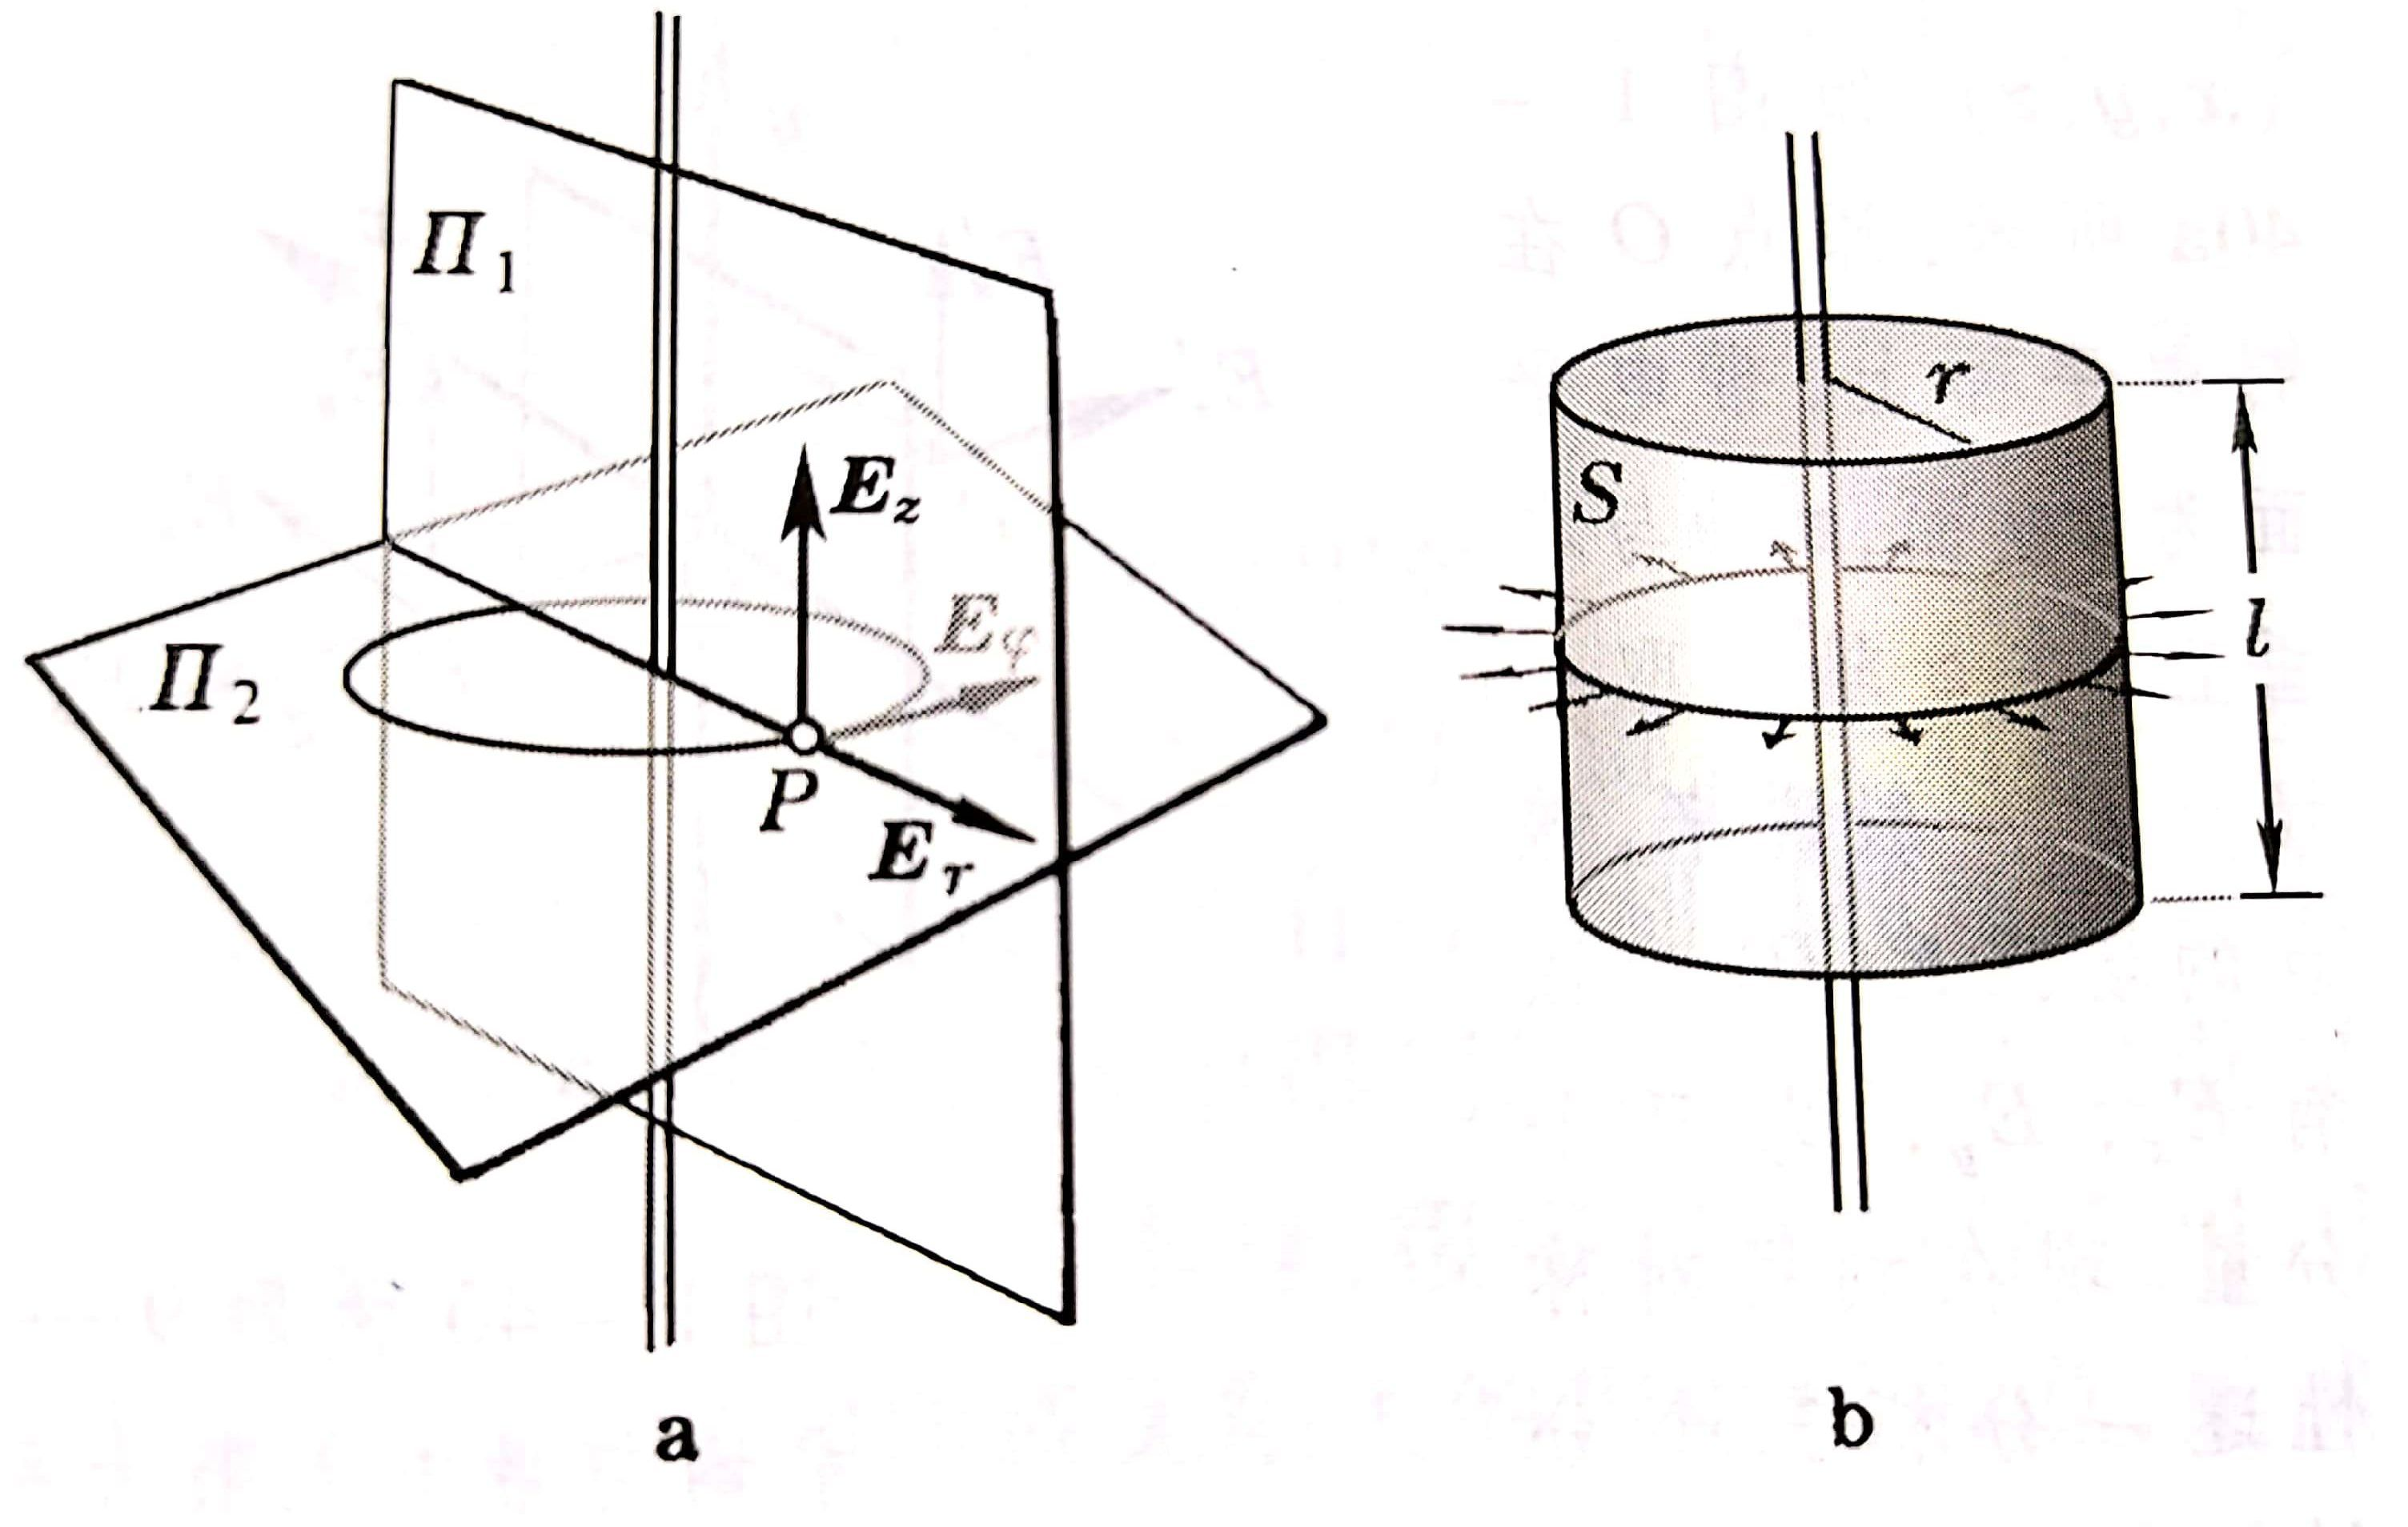
\includegraphics[width=0.8\textwidth]{hw2-p4-sketch.jpg}
    \caption{Sketches of Problem 4}
    \label{fig:4-sketch}
\end{figure}

We now may discuss the symmetry of this cylinder.

Since the cylinder is symmetric about plane $\Pi_1$, thus the electric field formed by the cylinder is symmetric about plane $\Pi_1$ as well. However, the direction of component $E_\varphi$ becomes reverse. Therefore, if and only if $E_\varphi$ = 0 can the cylinder obey the symmetry principle.

Analogously, since the cylinder is symmetric about plane $\Pi_2$, thus the electric field formed by the cylinder is symmetric about plane $\Pi_2$ as well. However, the direction of component $E_z$ becomes reverse. Therefore, if and only if $E_z$ = 0 can the cylinder obey the symmetry principle.

Hence the only component that is not equal to 0 is $E_r$. Since the cylinder has a constant bulk charge density($\rho$), points have as the same magnitude of electric field as those have the same distance from the middle axis. The sketch of electric field formed by this cylinder is shown in Fig. \ref{fig:4-sketch}b.

Then we get to calculate the \textbf{electric flux} first.

Suppose we take the surfaces of a piece of a cylinder whose length is $l$ as the \textbf{Gaussian surface}.
Since the base surfaces are parallel to the electric field, the electric flux $\Phi_E(base)$ = 0. The side surface is perpendicular to the electric filed.

\begin{enumerate}[(i)]
\item $r > R$
\begin{align}
    \Phi_E = \Phi_E(base) + \Phi_E(side) = 0 + 2\pi r l E = 2\pi r l E
\end{align}
Meanwhile, according to \textbf{Gauss's Law}
\begin{align}
    \Phi_E = \frac{Q}{\varepsilon_0} = \frac{\rho \pi R^2 l}{\varepsilon_0}
\end{align}
Hence
\begin{align}
    E = \frac{\rho R^2}{2\varepsilon_0 r}
\end{align}
Namely
\begin{align}
    \textbf{E} = \frac{\rho R^2}{2\varepsilon_0 r} \hat{\textbf{r}}
\end{align}

\item $r \leq R$

Analogously, we get
\begin{align}
    \frac{\rho \pi r^2 l}{\varepsilon_0} = 2\pi r l E
\end{align}
Hence
\begin{align}
    E = \frac{\rho r}{2\varepsilon_0}
\end{align}
Namely
\begin{equation}
    \textbf{E} = \frac{\rho r}{2\varepsilon_0} \hat{\textbf{r}}
    \label{4-eq}
\end{equation}
\end{enumerate}

Therefore, we conclude that
\begin{align*}
    \textbf{E} = 
    \left\{
        \begin{array}{lcl}
            \frac{\rho R^2}{2\varepsilon_0 r} \hat{\textbf{r}} & & (r > R) \\
              \\
            \frac{\rho r}{2\varepsilon_0} \hat{\textbf{r}} & & (r \leq R)
        \end{array}
    \right.
\end{align*}

Required sketch is shown below.
\begin{figure}[!htpb]
    \centering
    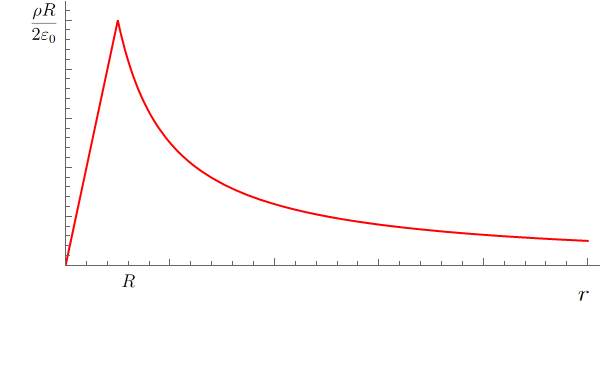
\includegraphics[width=0.6\textwidth]{hw2-p4-plot.png}
    \caption{Plot pf Problem 4}
    \label{fig:4-plot}
\end{figure}

\section*{\large \textbf{Problem 6}}~{\textbf{Solution}}

We may regard this stuff as an infinite cylinder with a uniform bulk density $\rho$ composed with a smaller infinite cylinder with a uniform bulk density -$\rho$. Based on \textbf{Problem 4}, we know
\begin{align}
    \textbf{E} = \frac{\rho}{2\varepsilon_0} \hat{\textbf{r}}
\end{align}

Hence for every point within that hole
\begin{align}
    \textbf{E} = \frac{\rho}{2\varepsilon_0} \left( \textbf{r}_1 - \textbf{r}_2 \right)
\end{align}
where $\textbf{r}_1$, $\textbf{r}_2$ denote the vector pointing from the point to the center of two cylinders correspondingly. Thus it is trivial that the electric fields in the hole are the same since $\textbf{r}_1$ - $\textbf{r}_2$ = \textbf{b} where \textbf{b} denotes the vector pointing from the center of the hole to the center of the bigger cylinder.

Namely
\begin{align}
    \textbf{E} = \frac{\rho}{2\varepsilon_0} \textbf{b}
\end{align}
which is uniform in the hole.

\section*{\large \textbf{Problem 7}}~{\textbf{Solution}}

\begin{enumerate}[(a)]
    \item
    \begin{align}
        q_a &= 4\pi r_a ^2 \sigma_a \\
        q_b &= 4\pi r_b ^2 \sigma_b \\
        q_a + q_b &= 4\pi R^2 \sigma_R
    \end{align}
    
    Thus we get
    \begin{align}
        \sigma_a &= \frac{q_a}{4\pi r_a ^2} \\
        \sigma_b &= \frac{q_b}{4\pi r_b ^2} \\
        \sigma_R &= \frac{q_a + q_b}{4\pi R^2}
    \end{align}
    
    \item For any point with a distance $r$ from the center of the neutral conducting ball, we set the \textbf{Gaussian surface} as the sphere with radius $r$, sharing the same center with the neutral conducting ball. Then according to \textbf{Gauss's Law}
    \begin{align}
        E(r) \cdot 4\pi r^2 = \frac{q_a + q_b}{\varepsilon_0}
    \end{align}
    
    Hence
    \begin{align}
        E(r) = \frac{q_a + q_b}{4\pi \varepsilon_0 r^2}
    \end{align}
    
    \item Analogously, we know
    \begin{align}
        E_a(r) \cdot 4\pi r_a ^2 &= \frac{q_a}{\varepsilon_0} \\
        E_b(r) \cdot 4\pi r_b ^2 &= \frac{q_b}{\varepsilon_0}
    \end{align}
    
    Hence
    \begin{align}
        E_a(r) &= \frac{q_a}{4\pi \varepsilon_0 r_a ^2} \\
        E_b(r) &= \frac{q_b}{4\pi \varepsilon_0 r_b ^2}
    \end{align}
    
    \item According to \textbf{Electrostatic Shield Effect}, the force between $q_a$ and $q_b$ will be zero.
    
    \item As an relatively in part, properties related to $q_a$ and $q_b$ individually will not change. However, the ball as a whole will change its property after adding $q_c$. \\
    Hence the surface densities of charge $\sigma_a$, $\sigma_b$, the electric field within each cavity and the force on $q_a$ and $q_b$ will not change while the surface density of the ball $\sigma_R$ and the electric field outside the conductor will change.
\end{enumerate}

\end{document}